% ---------------------------------------------------------------------------
\section{The method}
\label{sec:method}
% ---------------------------------------------------------------------------

HyperCommon has two settings: the commonality function $f$, which scores a pair of
nodes (closed-neighbourhood Jaccard unless stated otherwise), and the threshold $t$.
Given a graph $G$:
\begin{enumerate}
\item For every wedge $\{i,j,\ell\}$ -- three nodes, one adjacent to the other two,
  each counted once whether open or closed -- compute $f$ on its three pairs.
\item Admit the wedge as a hyperedge if all three values are at least $t$.
\item Join two admitted triples when they share two nodes, and return, for every
  connected component, the union of its triples' nodes.
\end{enumerate}
Commonality values are memoised per pair, and components are found on the bipartite
incidence graph between admitted triples and the pairs they contain, which has the
same triple components as the two-node-overlap graph and is linear in the number of
triples. Because the triple scores $s(T)=\min f$ over the pairs of $T$ do not depend on
$t$, the covers for every threshold follow from a single enumeration, each at the cost
of one component search. The threshold can be set from the graph alone, by maximising
the overlapping modularity of the cover~\cite{shen2009detect} (Sec.~\ref{sec:protocols}).
A local variant grows the community of a given seed triple by breadth-first search over
shared pairs, reading only the neighbourhoods of the nodes it reaches and of the
candidates it examines (Proposition~\ref{prop:local}).

\begin{figure*}[t]
  \centering
  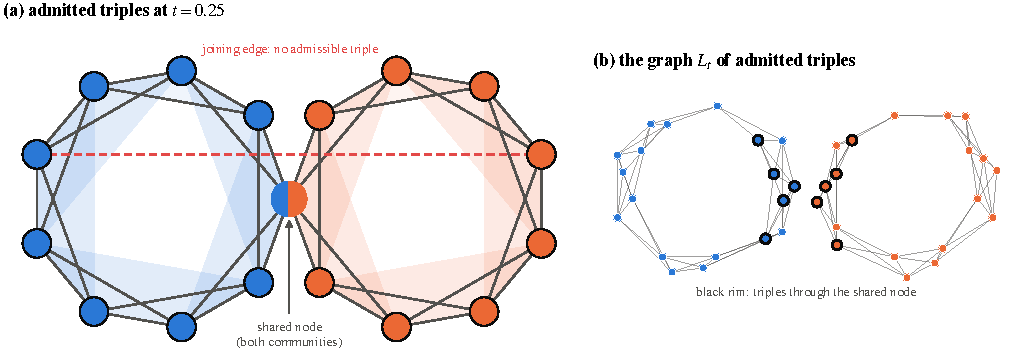
\includegraphics[width=0.85\textwidth]{figures/fig_schematic.pdf}
  \caption{The method on a toy graph, computed by the implementation. (a)~Two ring
  lattices of nine nodes ($k=4$) share one node, and one edge, placed by hand for the
  illustration between two nodes far from the shared node (it closes no triangle with
  it), joins them. Shaded triangles are the triples admitted at $t=0.25$, coloured by
  component; the shared node is admitted in both, the joining edge in none. (b)~The
  graph of admitted triples, linked when they share a pair ($L_t$), each component drawn
  on its own circle; its two components are the two communities. The rings have
  $s=9<2k+2$, outside the stated hypothesis of Theorem~\ref{thm:window} but within the
  ring sizes for which its window still holds (Sec.~\ref{app:proofsmore}).}
  \label{fig:schematic}
\end{figure*}

Figure~\ref{fig:schematic} illustrates the construction. Nodes in no admitted triple
remain unassigned, and communities have at least three members: the method reports only
what local evidence supports (coverage in Table~\ref{tab:S-coverage-label-free} of the
Supplemental Material~\cite{supplement}).
